\chapter{Physical Layer}
\label{cha:Physical Layer}
The physical layer is responsible for sending and receiving data to and from the network nodes. It is the component that makes the system communicate with the outside world. This layer can use different transmission technologies, for example, backscatter communication or Visible light communication.

\section{Implementation idea}
\label{sec:Implementation idea Phy}
The basic implementation idea was to develop a physical layer that would send bit-by-bit information on a single GPIO pin without the aid of external protocols such as UART, SPI, or I2C in such a way as to take advantage of a backscatter channel.\\
In practice, this implementation is a bit complicated, as it would be necessary to be able to generate interrupts for both rising and falling edges of the GPIO pin, then start a timer and periodically read the value of the pin by recording whether it is at logic level high (a "1" is being received) or low (a "0" is being received). This implementation idea needs synchronization and a fixed frequency transmission and reception; in fact, you need to know how often to sample the GPIO pin value.\\
  \begin{figure}[H]
    \centerline{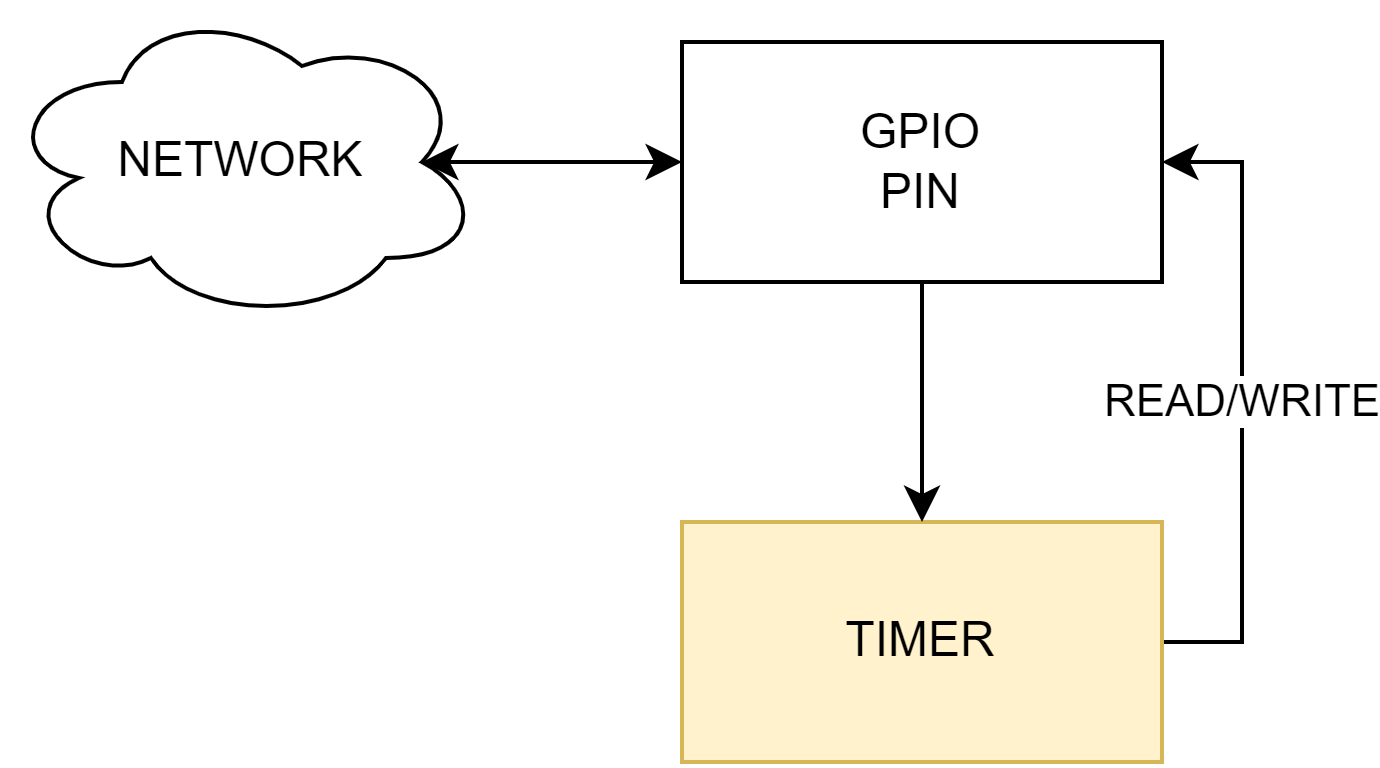
\psfig{file=Images/PhysicalReadIdealApproach.png,width=0.45\textwidth}}
    \caption{\footnotesize \centering Physical Layer implementation idea}
    \label{fig:PhysicalReadIdealApproach}
  \end{figure}

\section{Layer diagram}
\label{sec:Layer diagram Phy}
As can be understood, the architecture of the physical layer is not particularly complex: it receives data from the communication layer and broadcasts it to the network, and receives broadcast data from the network and forwards it to the communication layer. It can thus be schematized as follows:
  \begin{figure}[H]
    \centerline{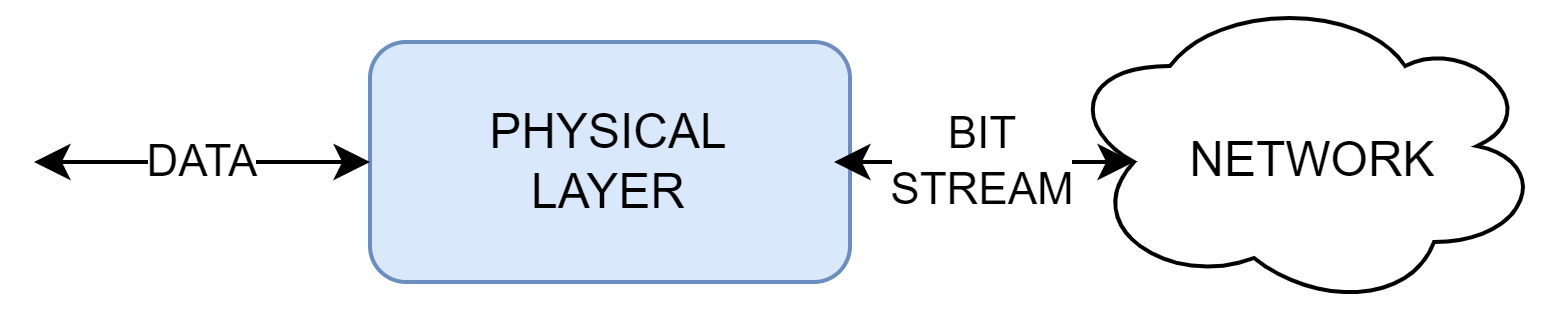
\psfig{file=Images/PhysicalLayerDiagram.png,width=0.5\textwidth}}
    \caption{\footnotesize \centering Physical Layer diagram}
    \label{fig:PhysicalLayerDiagram}
  \end{figure}

\section{Real implementation of the layer}
\label{sec:Real implementation of the layer Phy}
In the first section of this chapter, a possible implementation of the layer was provided. However, the proposed implementation is particularly complex to implement in practice.
Therefore, the choice was to use one of the UART modules on the MSP430 board to manage the sending and receiving of packets. 
The UART (Universal Asynchronous Receiver-Transmitter) module enables asynchronous communication that is not dependent on a synchronized clock and operates in full-duplex mode if necessary. It needs a dedicated TX output and RX input, which can be identified on the datasheet of the board.
Before the start of sending and receiving data, is needed to set the UART module to the desired baud rate. The baud rate indicates the transmission rate. Since is not present a shared clock it is necessary to have the same baud rate on the transmitting node and the receiving node to know how often to send and sample the signal.
For this project, the UART module was set to have a baud rate of 115200 b/s and send one byte at a time of data plus two bits to notify the start and end of the transmission.
The code below was used to achieve this configuration by taking the SMCLK (Sub-system master clock) set to 1MHz as the clock for baudrate generation.
\begin{lstlisting}
    //UART settings for BaudRate 115200 with 1MHz clock speed
    P2SEL0 &= ~(BIT5 | BIT6);
    P2SEL1 |= (BIT5 | BIT6);

    UCA1CTLW0 = UCSWRST;            //Put module in reset
    UCA1CTLW0 |= UCSSEL__SMCLK;
    UCA1BRW = 8;
    UCA1MCTLW = 0xD600;
    UCA1CTLW0 &= ~UCSWRST;          //Restore module from reset

    UCA1IE |= UCRXIE;               //Activate interrupt on module
\end{lstlisting}
RX TODO\\
TX TODO\\
  
\newpage




